While the model should be able to stand alone to represent the CubeSat system, stakeholders may prefer to view system details in document form. This could be because they don't have access to the modeling tool, or because they are more accustomed to seeing traditional reports. Whatever the reason, it would save time if those documents could be generated from model elements alone. Copying diagrams into a word processor and transcribing the requirements, etc. into tables, as is traditionally done, causes issues with version control and maintaining consistency. For example, if a team is writing a Space Vehicle Requirements Document, they could copy the requirement text from the model into a table in Microsoft Word, but if a requirement changes within the model, the team would need to catch that change and manually update any documents as a result. This CubeSat Reference Architecture proposes a new method for generating documents using Apache's Velocity Template Language. Cameo Systems Modeler is written in Java, so each model element is defined using Java code. This can be taken advantage of by populating a Microsoft Word file with code that imports those Java elements when it's run. Essentially, the Word templates tell Cameo what elements to export and in what order and in what format. This allows for fully custom, well-designed documents to be generated that require minimal formatting before delivery to stakeholders. If any model elements change, the team can just regenerate the document, and all tables, diagrams, etc. will always reflect the latest version that resides in the model. 

Figure \ref{fig:Document Generators} shows an organizational diagram showing the pre-built generators that are used in AFIT's Spacecraft Design Sequence. Instructions are also included, and an in-depth, commented Generic Model Document is provided. This generic document is the foundation for all other templates. This generic document has code for any Reference Architecture section and guidance for how to modify it and why the code is written the way it is. If a new document is requested that does not have a template yet, a team can take portions from this master document into a new template for whatever model elements they wish to display. It also maintains a revision history that resides in the model, so when changes are made, the team can notate those and they will show up in all future documents in a table of revisions. 

\begin{figure}[H]
    \centering
    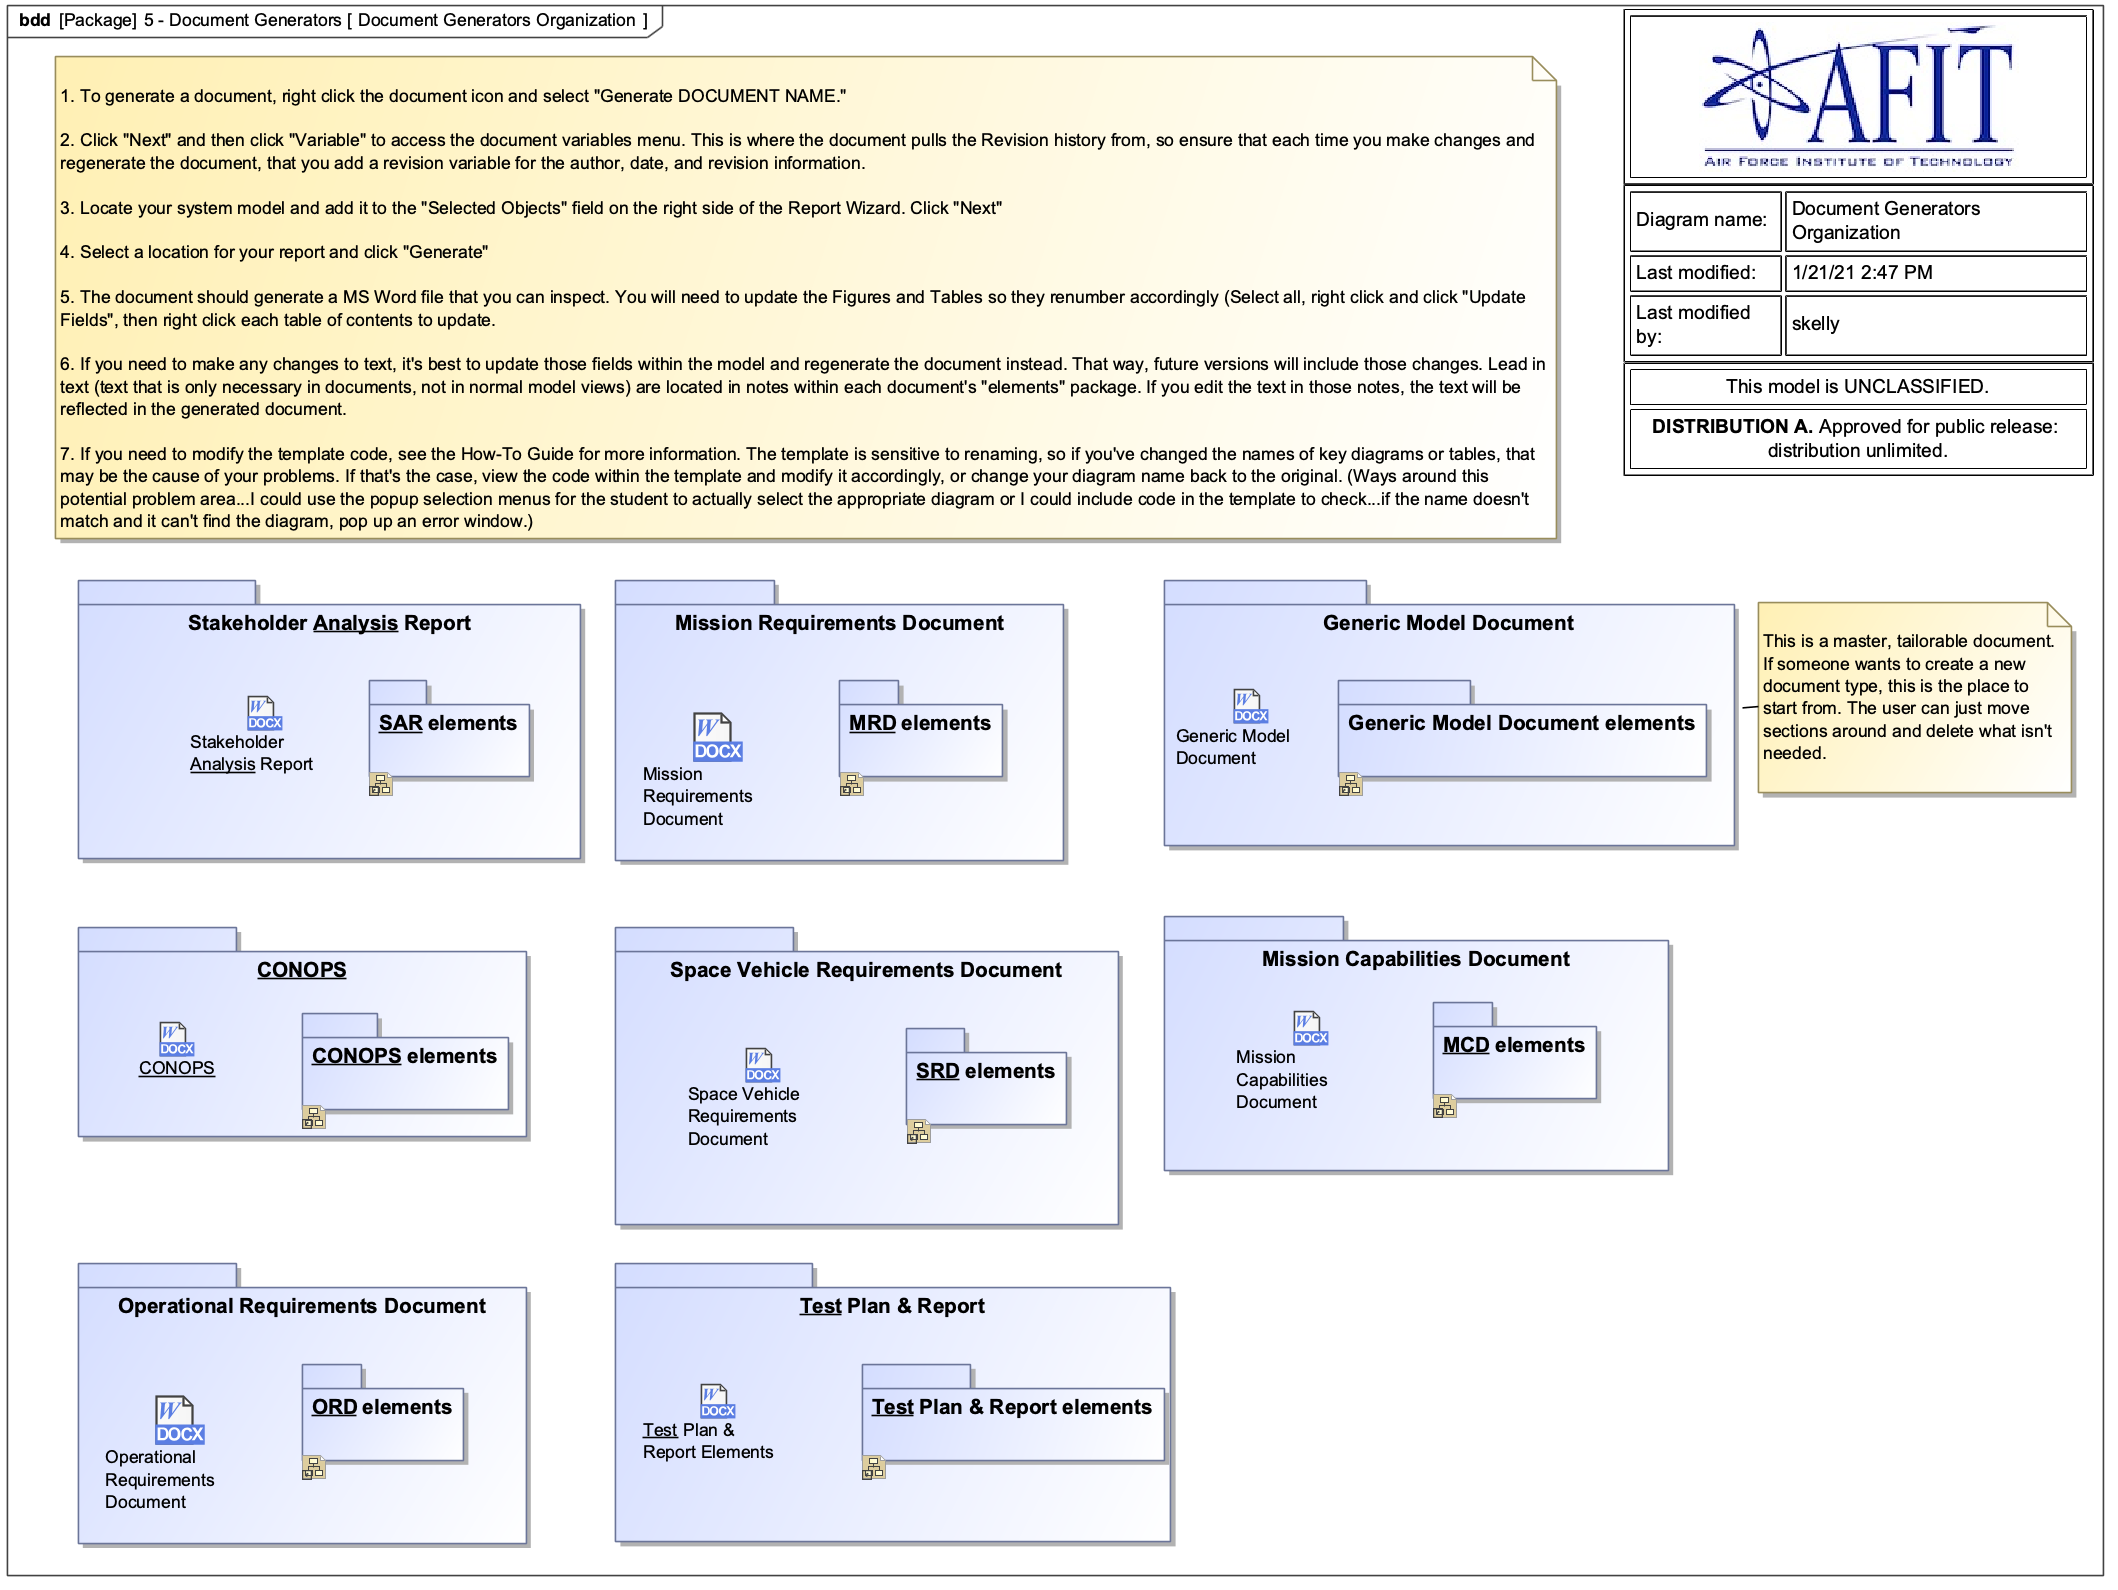
\includegraphics[width=\textwidth]{Thesis/Analysis_and_Results/Analysis and Results Figures/Document Generators.png}
    \caption{Document Generators}
    \label{fig:Document Generators}
\end{figure}

The title page of each template includes some custom functions that make the following code easier to write. Figure \ref{fig:Document Generator Title Page} shows several of these tools that are imported, allowing for tables to be easily exported and allowing for custom popup dialog prompts if a document generator should ask for a diagram's location. In this example, notice how a popup window asks the user to select their project's logo from among the model's free form diagrams, which is then imported by \$diagram.image. Code that follows a "\#" or "\$" is not displayed in the resulting document once it runs. Some variables, such as \$DocumentTitle, \$Classification, and \$Revisions are variables that are stored with the template, while others, such as \$missionRequirement are pulling each model element with that stereotype assigned to it. Note that in the Reference Architecture, the "Mission\_Requirement" stereotype is read by Java as the "missionRequirement" class. To prevent issues if users rename stereotypes, this practice has been minimized, opting instead to just import tables in their entirety when possible.

\begin{figure}[H]
    \centering
    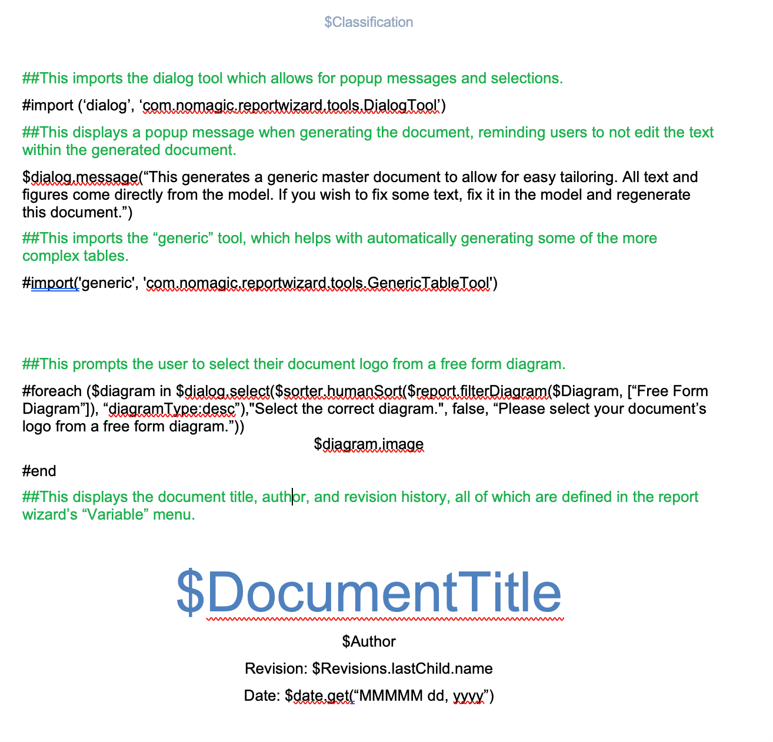
\includegraphics[width=\textwidth]{Thesis/Analysis_and_Results/Analysis and Results Figures/Document Generator Title Page.png}
    \caption{Document Generator Title Page}
    \label{fig:Document Generator Title Page}
\end{figure}

One of the most common functions within these document generators is importing tables from the model and displaying it using Microsoft Word's table tool. Some tables in the model are quite large and hard to read if they are copied and pasted onto a document, so these templates call the internal elements instead and display them in a way that's very easy to customize. Figures \ref{fig:Table Method 1} and \ref{fig:Table Method 2} show two ways to import and display tables. Figure \ref{fig:Table Method 1} shows a more detailed method to pull only the specific columns you want, which might be useful for very large tables. This method also allows for default column widths to reduce formatting once it is generated. This does present issues if users were to rename the "missionRequirement" class, as the code wouldn't find anything to import. The comments in the code should make it clear if someone opens the template to troubleshoot, but this is still a risk present using this method.

\begin{figure}[H]
    \centering
    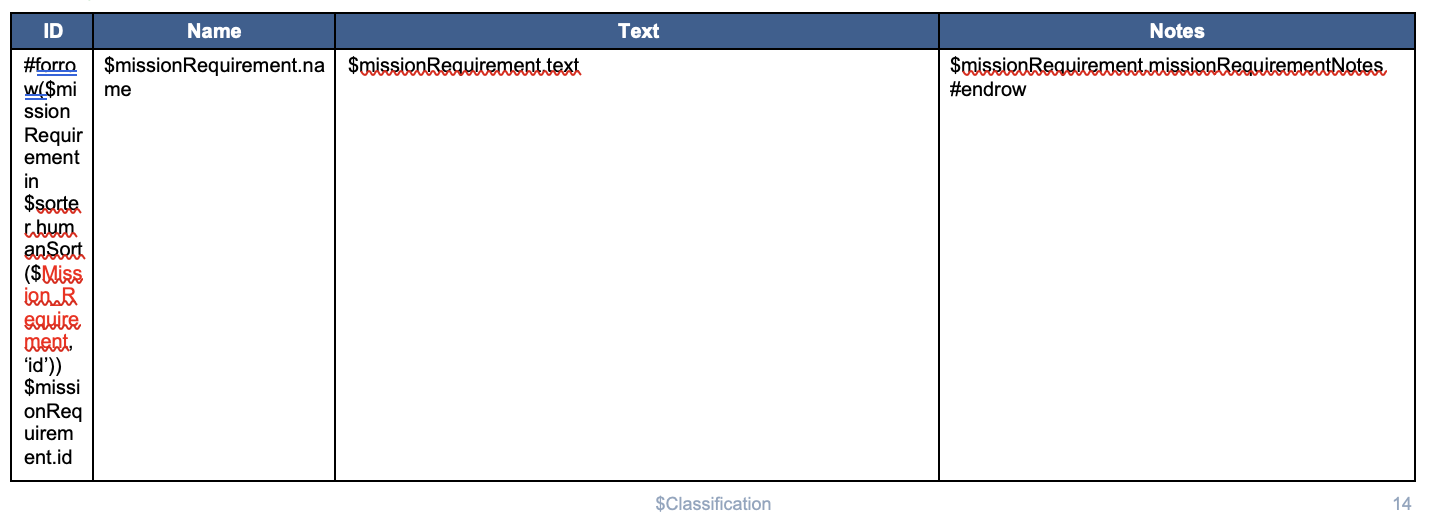
\includegraphics[width=\textwidth]{Thesis/Analysis_and_Results/Analysis and Results Figures/MR table method 1.png}
    \caption{Manual Table Method}
    \label{fig:Table Method 1}
\end{figure}

Figure \ref{fig:Table Method 2} shows a more elegant solution, where the template imports a table by name and displays it exactly as it appears in the model. The downside with this method is that it requires some modifications once it is generated, as columns will all be equally sized. Furthermore, some extra columns may be shown that are not desired, but these can be easily deleted. This method is preferred throughout the included templates as it is less likely to require modifications. It also displays new columns that users may wish to add without requiring an understanding of the VTL language to import those new elements.

\begin{figure}[H]
    \centering
    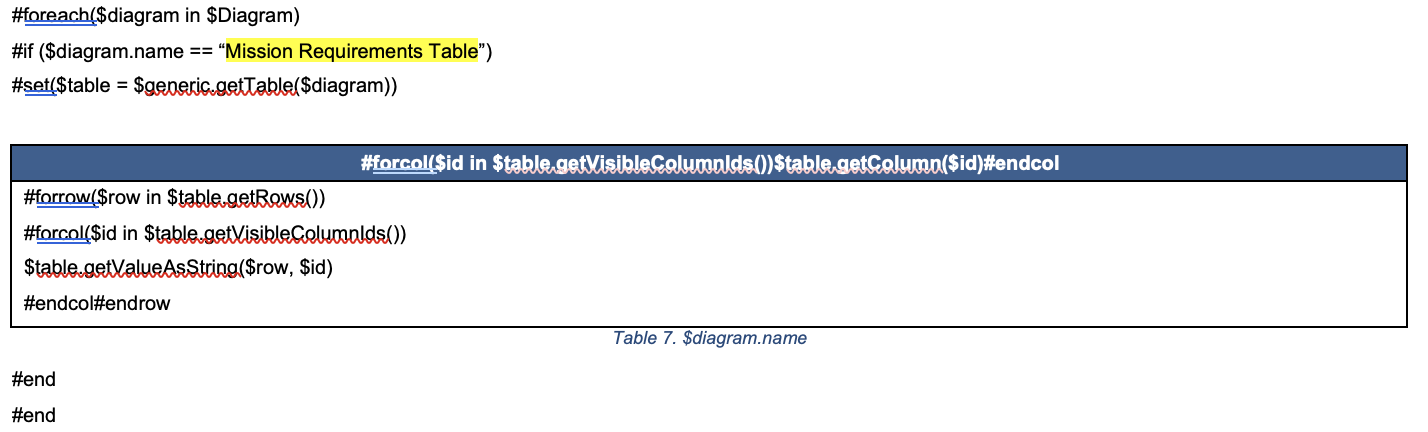
\includegraphics[width=\textwidth]{Thesis/Analysis_and_Results/Analysis and Results Figures/MR table method 2.png}
    \caption{Automatic Table Method}
    \label{fig:Table Method 2}
\end{figure}